\begin{frame}[t]{Otros comandos útiles}
    \begin{comando}
        git rm
    \end{comando}

    \only<2->{
        \begin{block}{}
            Permite borrar un archivo y marcarlo como \textit{preparado}. La sintaxis es \texttt{git rm [archivo]}
        \end{block}
    }

    \vspace{2em}

    \begin{comando}
        git mv
    \end{comando}

    \only<3->{
        \begin{block}{}
            Permite mover/renombrar un archivo y marcarlo como \textit{preparado}. La sintaxis es \texttt{git mv [archivo] [nuevo nombre/ubicación]}
        \end{block}
    }
\end{frame}

\begin{frame}[t]{Inspeccionando los cambios}
    \begin{comando}
        git diff
    \end{comando}

    \begin{block}{}
        Muchas veces es conveniente ver cuales son los cambios realizados antes de marcarlos como \textit{preparados}.

        Para esto tenemos el comando \texttt{git diff}, que muestra las diferencias entre lo que hay en
        tu directorio de trabajo con lo que hay en tu área de preparación.

        \vspace{1em}

        Si en cambio, queremos ver los cambios que preparamos y que irán en la próxima confirmación, podemos usar \texttt{git diff --staged}.
    \end{block}
\end{frame}

\begin{frame}[t]{Viendo la historia de los commits}
    \begin{comando}
        git log
    \end{comando}

    \pause
    \begin{block}{}
        Después de haber hecho varios \textit{commits}, o si acabamos de clonar un repositorio
        de internet, puede que querramos ver el historial de commits para ver cuales
        fueron las modificaciones que se hicieron. Esto se puede lograr utilizando el
        comando \texttt{git log}.
    \end{block}
\end{frame}

\begin{frame}{Ramificaciones en Git}

    Cada vez que realizamos una confirmación (commit), Git almacena entre otras cosas uno o varios punteros a las confirmaciones que
    sean padres directos de esta.

    Una rama o branch en Git no es más que un puntero especial parado en un commit. Ejecutar \texttt{git branch} nos mostrará las ramas actuales. Veamos un ejemplo sencillo:

    %\begin{columns}
    %    \column{0.5\textwidth}
    %    \begin{figure}[ht]
    %        \begin{center}
    %            \includegraphics[height=1.1in]{images/branch-and-history.png}
    %        \end{center}
    %        \caption{La rama ``master'' apunta al commit \textit{f30ab}}
    %    \end{figure}
    %    \column{0.5\textwidth}
    %    \begin{figure}[ht]
    %        \begin{center}
    %            \includegraphics[height=1.1in]{images/head-to-master.png}
    %        \end{center}
    %        \caption{Creamos una nueva rama ejecutando \texttt{git branch testing}}
    %    \end{figure}
    %\end{columns}

\end{frame}

\begin{frame}{Cambiando de rama}

    %\begin{figure}[ht]
    %    \begin{center}
    %        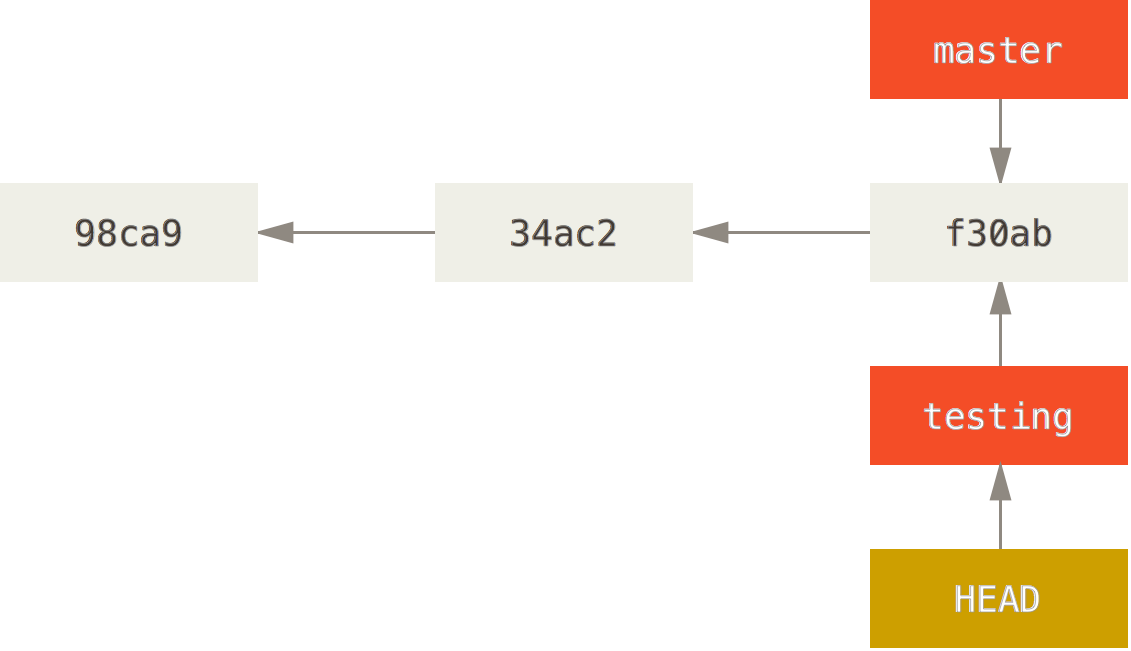
\includegraphics[height=1in]{images/head-to-testing.png}
    %    \end{center}
    %    \caption{Si queremos cambiar de rama, podemos ejecutar \texttt{git checkout testing}}
    %\end{figure}
    %\begin{figure}[ht]
    %    \begin{center}
    %        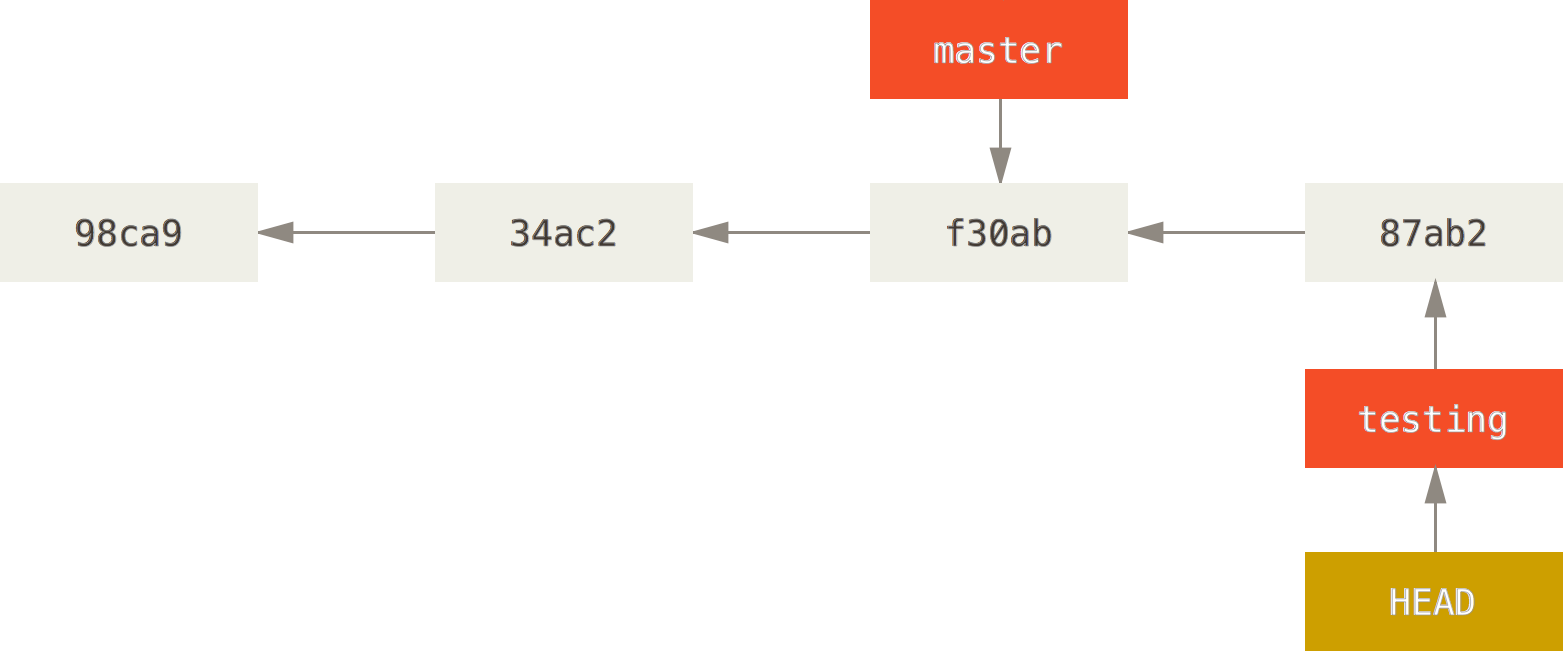
\includegraphics[height=1in]{images/advance-testing.png}
    %    \end{center}
    %    \caption{Y los siguientes commits serán agregados a la rama ``testing''}
    %\end{figure}

\end{frame}

\begin{frame}{Ramas remotas}

    Ademas de tener ramas locales, podemos tenemos ramas remotas, que referencian al estado de ramas en tus repositorios remotos.
    Si por ejemplo quisieramos saltar a la rama ``master'' en el repositorio remoto ``origin'' podríamos utilizar el comando \texttt{git checkout origin/master}.

    \vspace{1em}

    Nuestras ramas locales no sincronizan automaticamente con los repositorios remotos. Por esta razón, si tenemos una rama llamada ``master'' de forma local que
    apunta a la rama remota ``origin/master'' podemos actualizarla parandonos en ``master'' y ejecutando \texttt{git pull origin master}.

    \vspace{1em}

    De forma análoga, si queremos publicar cambios locales aun repositorio remoto, tenemos el comando \texttt{git push}. Si estamos parados en la rama ``master'':
    \texttt{git push origin master}.

\end{frame}

\begin{frame}{Fusionando ramas}

    Supongamos que tenemos una rama ``iss53'' en la cual hemos terminado de arreglar un error, y queremos combinarla con la rama ``master''.
    Para ello, simplemente nos paramos en ``master'' (\texttt{git checkout master}) y ejecutamos: \texttt{git merge iss53}.

	%\begin{figure}[ht]
	%	\begin{center}
	%		\includegraphics[height=1.5in]{images/basic-merging-1.png}
	%	\end{center}
	%	\caption{Antes del merge}
	%\end{figure}

\end{frame}

\begin{frame}{Fusionando ramas}

    Supongamos que tenemos una rama ``iss53'' en la cual hemos terminado de arreglar un error, y queremos combinarla con la rama ``master''.
    Para ello, simplemente nos paramos en ``master'' (\texttt{git checkout master}) y ejecutamos: \texttt{git merge iss53}.

	%\begin{figure}[ht]
	%	\begin{center}
	%		\includegraphics[height=1.5in]{images/basic-merging-2.png}
	%	\end{center}
	%	\caption{Después del merge}
	%\end{figure}

\end{frame}

\begin{frame}{Otros comandos útiles}

    \begin{itemize}
        \item \texttt{git fetch [remote repository]}: para traer todos los datos de un repositorio remoto.
        \item \texttt{git reset}: para deshacer cambios, ya sea en el area de trabajo o en los commits.
        \item \texttt{git rm}: para borrar un archivo y pasarlo al area de preparación.
        \item \texttt{git mv}: para mover/renombrar un archivo y pasarlo al area de preparación.
        \item \texttt{git show}: muestra información de distintos objectos de Git: commits, tags, etc.
        \item \texttt{git stash}: guarda el estado del area de trabajo y lo limpia.
        \item \texttt{git rebase [branch]}: aplica todos los commits que difieren entre un branch y el que estamos parados.
        \item \texttt{git tag [etiqueta] [commit hash]}: ponerle una etiqueta a un commit.
    \end{itemize}

\end{frame}

\begin{frame}{Bibliografía extra}

    \begin{itemize}
        \item Git Community book, disponible online y en español: \url{https://git-scm.com/book/es/v2}
		\item \texttt{git help [command]} para ver la documentación de cualquier comando de Git.
		\item A visual Git reference: \url{http://marklodato.github.io/visual-git-guide/index-es.html}
		\item Try Git online: \url{https://try.github.io}
        \item Git - SVN Crash Course: \url{https://git-scm.com/course/svn.html}
    \end{itemize}

\end{frame}

\begin{frame}{Mini ejercicio de práctica}

	\begin{block}{Básico}
		\begin{enumerate}
			\item Instalar Git en tu máquina.
			\item Clonar el repositorio que tiene los fuentes de estas diapositivas. (git@github.com:FlyingPumba/git-intro.git)
			\item Abrir el archivo \textit{main.tex} y \textbf{arregkar} el typo en esta oración.
			\item Pasar \textit{main.tex} al area de preparados.
			\item Confirmar los cambios.
		\end{enumerate}
	\end{block}

\end{frame}


\begin{frame}{Mini ejercicio de práctica}

	\begin{block}{Avanzado}
		\begin{enumerate}
			\item Crearse una cuenta en \url{GitHub.com}
			\item Ir a la página del repositorio que tiene los fuentes de estas diapositivas \url{https://github.com/FlyingPumba/git-intro} y \textit{forkear} el proyecto a un repositorio personal en GitHub.
			\item Agregar a su repositorio local un nuevo remoto llamado ``fork'' que apunte a su repositorio remoto en GitHub.
			\item Pushear la rama ``master'' al repositorio remoto ``fork''.
			\item Hacer un \textit{Pull request} en GitHub.
		\end{enumerate}
	\end{block}

\end{frame}
